\chapter{Central Force Motion- Solutions}
\begin{abox}
	Practice set - 1 
	\end{abox}
\begin{enumerate}
		\item The acceleration due to gravity $(g)$ on the surface of Earth is approximately $2.6$ times that on the surface of Mars. Given that the radius of Mars is about one half the radius of Earth, the ratio of the escape velocity on Earth to that on Mars is approximately
		{\exyear{NET JUNE 2011}}
	\begin{tasks}(2)
		\task[\textbf{A.}] $1.1$
		\task[\textbf{B.}]$1.3$
		\task[\textbf{C.}]$2.3$
		\task[\textbf{D.}]$5.2$
	\end{tasks}
\begin{answer}
\begin{align*}
	\text { Escape velocity }&=\sqrt{2 g R}\\
\frac{\text { Escape velocity of Earth }}{\text { Escape velocity of Mass }}&=\sqrt{\frac{g_{e} R_{e}}{g_{m} R_{m}}}=2.3 \quad \text { where } \frac{R_{e}}{R_{m}}=2 \text { and } \frac{g_{e}}{g_{m}}=2.6
\end{align*}
	THe correct option is \textbf{(c)}
\end{answer}
	\item Two particles of identical mass move in circular orbits under a central potential $V(r)=\frac{1}{2} k r^{2}$. Let $l_{1}$ and $l_{2}$ be the angular momenta and $r_{1}, r_{2}$ be the radii of the orbits respectively. If $\frac{l_{1}}{l_{2}}=2$, the value of $\frac{r_{1}}{r_{2}}$ is:
	{\exyear{NET DEC 2011}}
\begin{tasks}(2)
	\task[\textbf{A.}] $\sqrt{2}$
	\task[\textbf{B.}]$1 / \sqrt{2}$
	\task[\textbf{C.}] 2
	\task[\textbf{D.}] $1 / 2$
\end{tasks}
\begin{answer}
	\begin{align*}
	 V_{e f f}&=\frac{l^{2}}{2 m r^{2}}+\frac{1}{2} k r^{2}, \text{where $l$ is angular momentum. }\\
	\intertext{Condition for circular orbit} \frac{\partial V_{e f f}}{\partial r}&=0 \Rightarrow-\frac{l^{2}}{m r^{3}}+k r=0 \Rightarrow l^{2} \propto r^{4} \Rightarrow l \propto r^{2}.\\
	Thus \frac{l_{1}}{l_{2}}&=\left(\frac{r_{1}}{r_{2}}\right)^{2} \Rightarrow \frac{r_{1}}{r_{2}}=\sqrt{\frac{l_{1}}{l_{2}}} \Rightarrow \frac{r_{1}}{r_{2}}=\sqrt{2}\\ 
	since \frac{l_{1}}{l_{2}}&=2
	\end{align*}
	The correct option is \textbf{(a)}
\end{answer}
	\item A planet of mass $m$ moves in the inverse square central force field of the Sun of mass $M$. If the semi-major and semi-minor axes of the orbit are $a$ and $b$, respectively, the total energy of the planet is:
	{\exyear{NET DEC 2011}}
\begin{tasks}(2)
	\task[\textbf{A.}] $-\frac{G M m}{a+b}$
	\task[\textbf{B.}]$-G M m\left(\frac{1}{a}+\frac{1}{b}\right)$
	\task[\textbf{C.}]$-\frac{G M m}{a}\left(\frac{1}{b}-\frac{1}{a}\right)$
	\task[\textbf{D.}]$-G M m\left(\frac{a-b}{(a+b)^{2}}\right)$
\end{tasks}
\begin{answer}
 Assume Sun is at the centre of elliptical orbit. Conservation of energy\\
  $$\frac{1}{2} m v_{1}^{2}-\frac{G M m}{a}=\frac{1}{2} m v_{2}^{2}-\frac{G M m}{b}$$ Conservation of momentum $L=m v_{1} a=m v_{2} b$\\
  \begin{figure}[H]
  	\centering
  	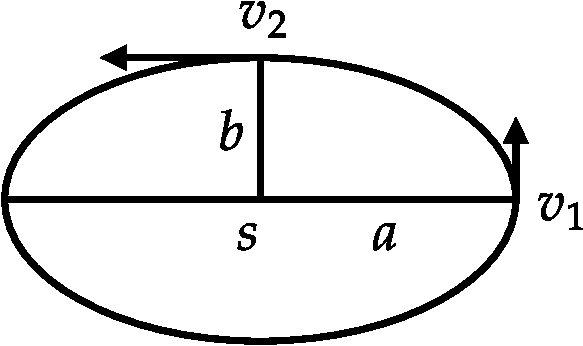
\includegraphics[height=3cm,width=5cm]{diagram-20210926(12)-crop}
  \end{figure}
 \begin{align*}
 	&v_{2}=v_{1}\left(\frac{a}{b}\right) \\
 	&\frac{1}{2} m v_{1}^{2}-\frac{1}{2} m v_{2}^{2}=\frac{G M m}{a}-\frac{G M m}{b} \Rightarrow \frac{1}{2} m\left(v_{1}^{2}-v_{1}^{2} \frac{a^{2}}{b^{2}}\right)=G M m\left(\frac{b-a}{a b}\right) \\
 	&\frac{1}{2} m v_{1}^{2}\left(\frac{b^{2}-a^{2}}{b^{2}}\right)=G M m\left(\frac{b-a}{a b}\right) \Rightarrow \frac{1}{2} m v_{1}^{2}=G M m\left(\frac{b}{a}\right) \cdot \frac{1}{(b+a)} \\
 	&E=\frac{1}{2} m v_{1}^{2}-\frac{G M m}{a}=G M m \frac{b}{a} \frac{1}{(b+a)}-\frac{G M m}{a} \\
 	&=\frac{G M m}{a}\left(\frac{b}{(b+a)}-1\right)=\frac{G M m}{a}\left(\frac{b-b-a}{(b+a)}\right)=-\frac{G M m}{(b+a)}
 \end{align*}
 The correct option is \textbf{(a)}	
\end{answer}

	\item A planet of mass $m$ moves in the gravitational field of the Sun (mass $M$ ). If the semimajor and semi-minor axes of the orbit are $a$ and $b$ respectively, the angular momentum of the planet is
	{\exyear{NET DEC 2012}}

\begin{tasks}(2)
	\task[\textbf{A.}]$\sqrt{2 G M m^{2}(a+b)}$
	\task[\textbf{B.}]$\sqrt{2 G M m^{2}(a-b)}$
	\task[\textbf{C.}]$\sqrt{\frac{2 G M m^{2} a b}{a-b}}$
	\task[\textbf{D.}]$\sqrt{\frac{2 G M m^{2} a b}{a+b}}$
\end{tasks}
\begin{answer}
	 Assume Sun is at the centre of elliptical orbit.\\\\
	Conservation of energy $\frac{1}{2} m v_{1}^{2}-\frac{G M m}{a}=\frac{1}{2} m v_{2}^{2}-\frac{G M m}{b}$\\\\
	Conservation of momentum $L=m v_{1} a=m v_{2} b$
	$$
	v_{2}=v_{1}\left(\frac{a}{b}\right)
	$$
	\begin{figure}[H]
		\centering
		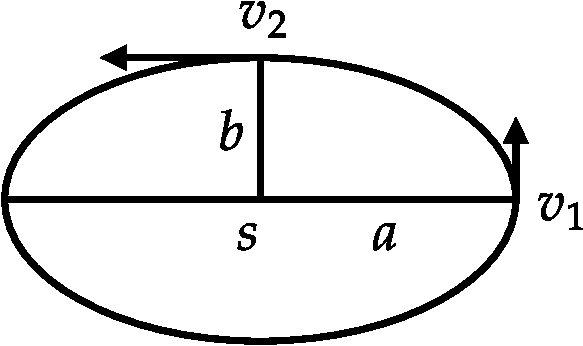
\includegraphics[height=3cm,width=5cm]{diagram-20210926(12)-crop}
	\end{figure}
	\begin{align*}
		&\frac{1}{2} m v_{1}^{2}-\frac{1}{2} m v_{2}^{2}=\frac{G M m}{a}-\frac{G M m}{b} \Rightarrow \frac{1}{2} m\left(v_{1}^{2}-v_{1}^{2} \frac{a^{2}}{b^{2}}\right)=G M m\left(\frac{b-a}{a b}\right) \\
		&\frac{1}{2} m v_{1}^{2}\left(\frac{b^{2}-a^{2}}{b^{2}}\right)=G M m\left(\frac{b-a}{a b}\right) \Rightarrow \frac{1}{2} m v_{1}^{2}=G M m\left(\frac{b}{a}\right) \cdot \frac{1}{(b+a)} \\
		&v_{1}=\sqrt{2 G M\left(\frac{b}{a}\right) \cdot \frac{1}{(b+a)}} \\
		&L=m v_{1} a=m \sqrt{2 G M\left(\frac{b}{a}\right) \cdot\left(\frac{1}{b+a}\right)} \cdot a=m \sqrt{\frac{2 G M a b}{(b+a)}} \Rightarrow L=\sqrt{\frac{2 G M m^{2} a b}{a+b}}
	\end{align*}
	The correct option is \textbf{(d)}
\end{answer}
	\item A planet of mass $m$ and an angular momentum $L$ moves in a circular orbit in a potential, $V(r)=-k / r$, where $k$ is a constant. If it is slightly perturbed radially, the angular frequency of radial oscillations is
	{\exyear{NET JUNE 2013}}
\begin{tasks}(2)
	\task[\textbf{A.}] $m k^{2} / \sqrt{2} L^{3}$
	\task[\textbf{B.}]$m k^{2} / L^{3}$
	\task[\textbf{C.}]$\sqrt{2} m k^{2} / L^{3}$
	\task[\textbf{D.}]$\sqrt{3} m k^{2} / L^{3}$
\end{tasks}
\begin{answer}$\left. \right. $\\
	\begin{minipage}{0.5\textwidth}
	\begin{align*}
	V_{e f f}&=\frac{L^{2}}{2 m r^{2}}-\frac{k}{r} \\
	\intertext{For circular orbit} \frac{\partial V_{e f f}}{\partial r}&=-\frac{L^{2}}{m r^{3}}+\frac{k}{r^{2}}=0 \\
	\Rightarrow \frac{L^{2}}{m r^{3}}&=\frac{k}{r^{2}} \\
	\text{Thus} r&=r_{0}=\frac{L^{2}}{m k} \Rightarrow \omega=\sqrt{\frac{k}{m}},
	\end{align*}
	\end{minipage}
\begin{minipage}{0.5\textwidth}
\begin{figure}[H]
	\centering
	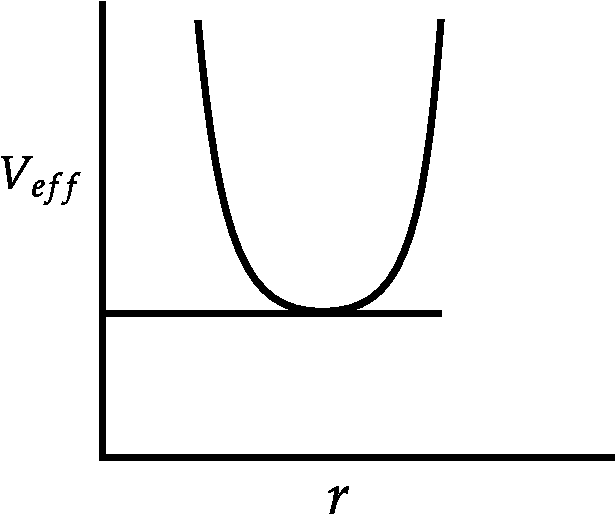
\includegraphics[height=4cm,width=5cm]{diagram-20210926(17)-crop}
\end{figure}
\end{minipage}
 \begin{align*}
 k&=\left.\frac{d^{2} V_{e f f}}{d r^{2}}\right|_{r=r_{0}}=+\frac{3 L^{2}}{m r^{4}}-\left.\frac{2 k}{r^{3}}\right|_{r=r_{0}}=\frac{3 L^{2}}{m\left(\frac{L^{2}}{m k}\right)^{4}}-\frac{2 k}{\left(\frac{L^{2}}{m k}\right)^{3}}=\frac{3 m^{3} k^{4}}{L^{6}}-\frac{2 m^{3} k^{4}}{L^{6}}=\frac{m^{3} k^{4}}{L^{6}}\\
 \omega&=\sqrt{\frac{\left.\frac{d^{2} V}{d r^{2}}\right|_{r=r_{0}}}{m}} \Rightarrow \omega=\frac{m k^{2}}{L^{3}}
 \end{align*}
 The correct option is \textbf{(b)}	
\end{answer}

\item The radius of Earth is approximately $6400 \mathrm{~km}$. The height $h$ at which the acceleration due to Earth's gravity differs from $g$ at the Earth's surface by approximately $1 \%$ is
	{\exyear{NET DEC 2014}}
\begin{tasks}(2)
	\task[\textbf{A.}] $64 \mathrm{~km}$
	\task[\textbf{B.}] $48 \mathrm{~km}$
	\task[\textbf{C.}]$32 \mathrm{~km}$
	\task[\textbf{D.}]$16 \mathrm{~km}$
\end{tasks}
\begin{answer}
$\frac{g}{g^{\prime}}=1+\frac{2 h}{R} \Rightarrow \frac{g}{g^{\prime}}-1=\frac{2 h}{R} \Rightarrow \frac{\Delta g}{g^{\prime}}=\frac{2 h}{R} \Rightarrow h=32 k \cdot m$\\
The correct option is \textbf{(c)}	
\end{answer}

	\item The probe Mangalyaan was sent recently to explore the planet Mars. The inter-planetary part of the trajectory is approximately a half-ellipse with the Earth (at the time of launch),Sun and Mars (at the time the probe reaches the destination) forming the major axis. Assuming that the orbits of Earth and Mars are approximately circular with radii $R_{E}$ and $R_{M}$, respectively, the velocity (with respect to the Sun) of the probe during its voyage when it is at a distance
		\begin{figure}[H]
		\centering
		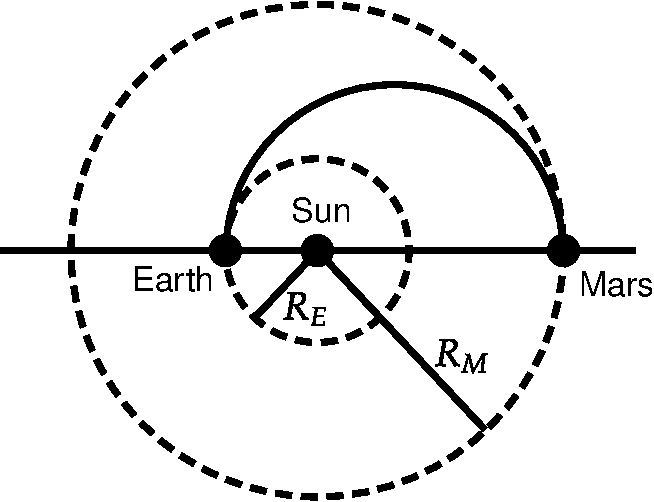
\includegraphics[height=3cm,width=5cm]{diagram-20210926(22)-crop(1)}
	\end{figure}
	 $r\left(R_{E}<<r<<R_{M}\right) \text { from the Sun, neglecting the effect of Earth and Mars, is }$
	{\exyear{NET DEC 2014}}
\begin{tasks}(2)
	\task[\textbf{A.}] $\sqrt{2 G M \frac{\left(R_{E}+R_{M}\right)}{r\left(R_{E}+R_{M}-r\right)}}$
	\task[\textbf{B.}]$\sqrt{2 G M \frac{\left(R_{E}+R_{M}-r\right)}{r\left(R_{E}+R_{M}\right)}}$
	\task[\textbf{C.}]$\sqrt{2 G M \frac{R_{E}}{r R_{M}}}$
	\task[\textbf{D.}]$\sqrt{\frac{2 G M}{r}}$
\end{tasks}
\begin{answer}
	$\text { Total energy } E=-K / 2 a \text { where } 2 a \text { major axis and } 2 a=R_{E}+R_{M} \text {. }$
	$$\frac{1}{2} m v^{2}-\frac{G M m}{r}=-\frac{G M m}{\left(R_{E}+R_{M}\right)} \Rightarrow v=\sqrt{2 G M \frac{\left(R_{E}+R_{M}-r\right)}{r\left(R_{E}+R_{M}\right)}}$$
	The correct option is \textbf{(b)}
\end{answer}
	\item After a perfectly elastic collision of two identical balls, one of which was initially at rest, the velocities of both the balls are non zero. The angle $\theta$ between the final, velocities (in the lab frame) is
	{\exyear{NET DEC 2016}}
\begin{tasks}(2)
	\task[\textbf{A.}] $\theta=\frac{\pi}{2}$
	\task[\textbf{B.}]$\theta=\pi$
	\task[\textbf{C.}]$0<\theta \leq \frac{\pi}{2}$
	\task[\textbf{D.}] $\frac{\pi}{2}<\theta \leq \pi$
\end{tasks}
\begin{answer}
 Angle between two particle $\theta_{1}+\theta_{2}=0$
Conservation of momentum
\begin{align*}
&m u=m v_{1} \cos \theta_{1}+m v_{2} \cos \theta_{2} \\
&0=m v_{1} \sin \theta_{1}-m v_{2} \sin \theta_{2}
\intertext{conservation of kinetic energy }
&\frac{1}{2} m u^{2}=\frac{1}{2} m v_{1}^{2}+\frac{1}{2} m v_{2}^{2}\\
	&u^{2}=v_{1}^{2}+v_{2}^{2}+2 v_{1} v_{2}\left(\cos \theta_{1} \cos \theta_{2}-\sin \theta_{1} \sin \theta_{2}\right) \\
	&u^{2}=v_{1}^{2}+v_{2}^{2}+2 v_{1} v_{2} \cos \left(\theta_{1}+\theta_{2}\right) \\
	&u^{2}=v_{1}^{2}+v_{2}^{2} \\
	&v_{1}^{2}+v_{2}^{2}=v_{1}^{2}+v_{2}^{2}+2 v_{1} v_{2} \cos \left(\theta_{1}+\theta_{2}\right) \\
	&\cos \left(\theta_{1}+\theta_{2}\right)=0 \\
	&\theta_{1}+\theta_{2}=\frac{\pi}{2} \Rightarrow \theta=\frac{\pi}{2}
\end{align*}
The correct option is \textbf{(a)}	
\end{answer}
	\item Consider circular orbits in a central force potential $V(r)=-\frac{k}{r^{n}}$, where $k>0$ and $0<n<2$. If the time period of a circular orbit of radius $R$ is $T_{1}$ and that of radius $2 R$ is $T_{2}$, then $\frac{T_{2}}{T_{1}}$
	{\exyear{NET DEC 2016}}
\begin{tasks}(2)
	\task[\textbf{A.}] $2^{\frac{n}{2}}$
	\task[\textbf{B.}]$2^{\frac{2}{3} n}$
	\task[\textbf{C.}]$2^{\frac{n}{2}+1}$
	\task[\textbf{D.}]$2^{n}$
\end{tasks}
\begin{answer}
	\begin{align*}
		&V_{e f f}=\frac{J^{2}}{2 m r^{2}}-\frac{k}{r^{n}}, \frac{\partial V_{e f f}}{\partial r}=-\frac{J^{2}}{m r^{3}}+\frac{n k}{r^{n+1}}=0\\
		&\because J=m r^{2} \omega \Rightarrow \frac{m^{2} \omega^{2} r^{4}}{r^{3}}=\frac{n k}{r^{n+1}} \Rightarrow \omega^{2} \propto \frac{1}{r^{n+2}} \Rightarrow \omega \propto r^{-(n+2) / 2} \Rightarrow T \propto r^{\frac{n}{2}+1} \\
		&\frac{T_{2}}{T_{1}}=\left(\frac{2 R}{R}\right)^{\frac{n+2}{2}}=2^{\frac{n}{2}+1}
	\end{align*}
	The correct option is \textbf{(c)}
\end{answer}
	\item A ball weighing $100 \mathrm{gm}$, released from a height of $5 \mathrm{~m}$, bounces perfectly elastically off a plate. The collision time between the ball and the plate is $0.5 \mathrm{~s}$. The average force on the plate is approximately
{	\exyear{NET JUNE 2017}}
\begin{tasks}(2)
	\task[\textbf{A.}] $3 N$
	\task[\textbf{B.}]$2 N$
	\task[\textbf{C.}]$5 N$
	\task[\textbf{D.}]$4 N$
\end{tasks}
\begin{answer}
\begin{align*}
m&=\frac{100}{1000}=0.1 \mathrm{~kg}\\
m g h&=\frac{1}{2} m v^{2} \\
v&=\sqrt{2 g h} \\
v & =10 \mathrm{~m} / \mathrm{sec}
\intertext{change in momentum during collision}
 (m v)-(-m v)&=2 k . g m / \mathrm{sec}\\
f&=\frac{\Delta P}{\Delta t}=\frac{2}{0.5}=4 N
\end{align*}
The correct option is \textbf{(d)}	
\end{answer}
	\item Which of the following figures best describes the trajectory of a particle moving in a repulsive central potential $V(r)=\frac{a}{r}(a>0$ is a constant)?
	{\exyear{NET JUNE 2018}}
\begin{tasks}(2)
	\task[\textbf{A.}]\begin{figure}[H]
		\centering
		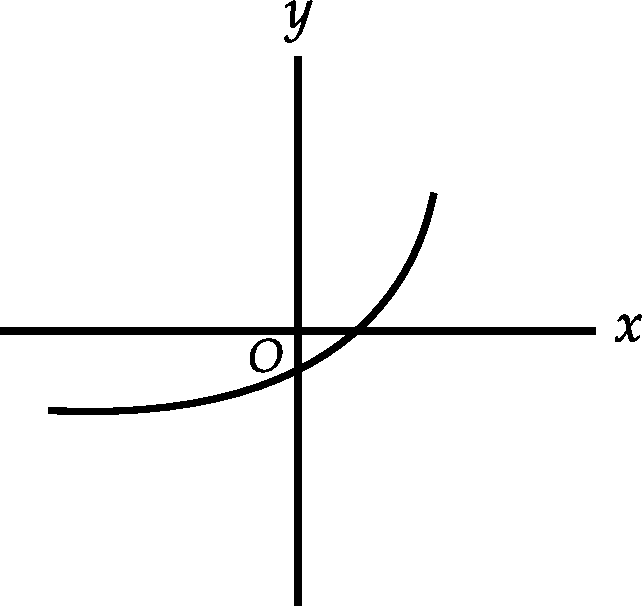
\includegraphics[height=3cm,width=5cm]{diagram-20210926(47)-crop}
	\end{figure}
	\task[\textbf{B.}]\begin{figure}[H]
		\centering
		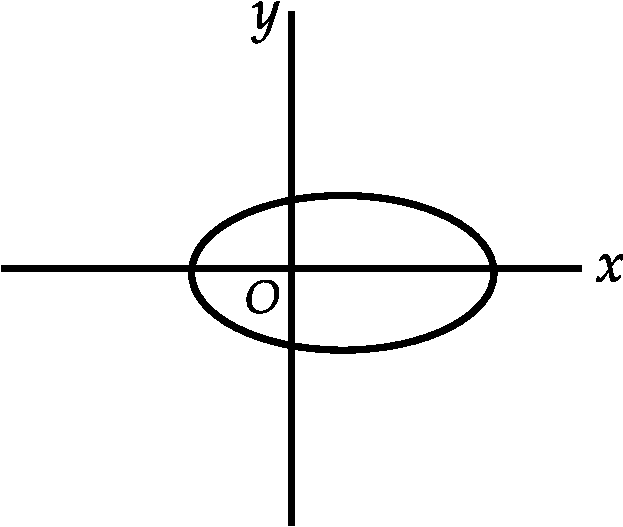
\includegraphics[height=3cm,width=5cm]{diagram-20210926(48)-crop}
	\end{figure}
	\task[\textbf{C.}]\begin{figure}[H]
		\centering
		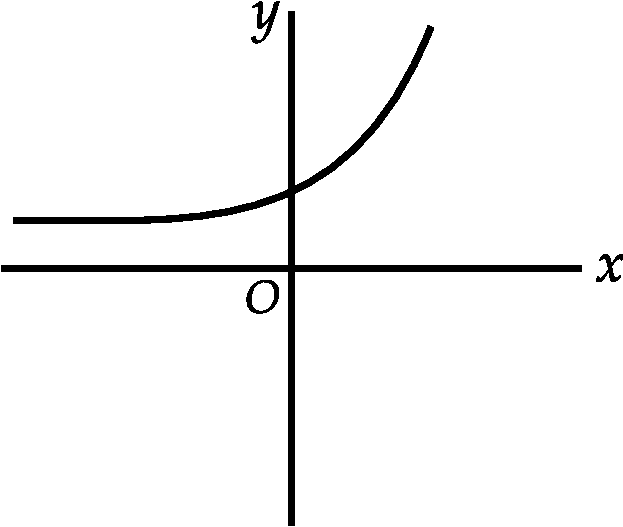
\includegraphics[height=3cm,width=5cm]{diagram-20210926(49)-crop}
	\end{figure}
	\task[\textbf{D.}]\begin{figure}[H]
		\centering
		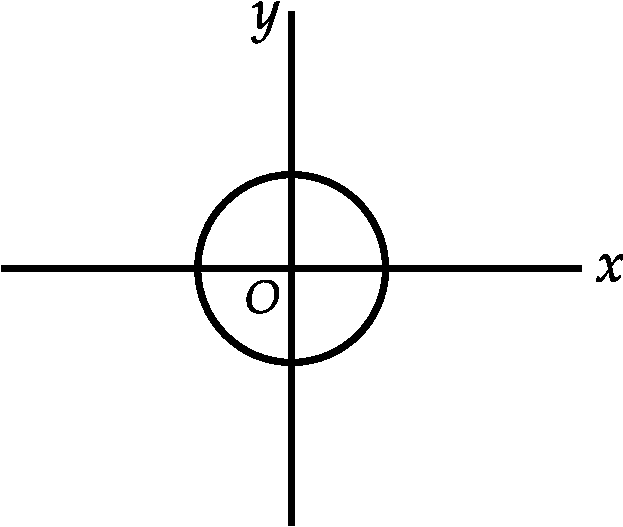
\includegraphics[height=3cm,width=5cm]{diagram-20210926(50)-crop}
	\end{figure}
\end{tasks}
\begin{answer}
\begin{minipage}{0.5\textwidth}
	 The potential is $V(r)=\frac{a}{r}$ which is repulsive. So there is unbounded motion and mainly represent by scattering project
\end{minipage}
\begin{minipage}{0.5\textwidth}
\begin{figure}[H]
	\centering
	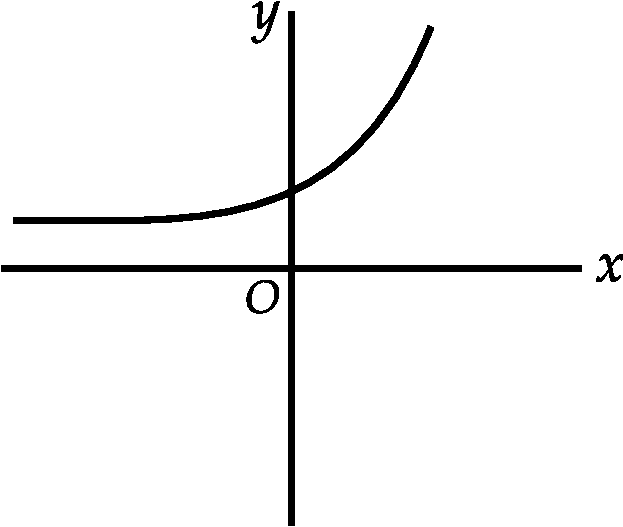
\includegraphics[height=3cm,width=5cm]{diagram-20210926(51)-crop}
\end{figure}
\end{minipage}\\
The correct option is \textbf{(c)}
\end{answer}

	\item A particle of mass $m$ moves in a central potential $V(r)=-\frac{k}{r}$ in an elliptic orbit $r(\theta)=\frac{a\left(1-e^{2}\right)}{1+e \cos \theta}$, where $0 \leq \theta<2 \pi$ and $a$ and $e$ denote the semi-major axis and eccentricity, respectively. If its total energy is $E=-\frac{k}{2 a}$, the maximum kinetic energy is
	{\exyear{NET JUNE 2018}}
\begin{tasks}(2)
	\task[\textbf{A.}] $E\left(1-e^{2}\right)$
	\task[\textbf{B.}]$E \frac{(e+1)}{(e-1)}$
	\task[\textbf{C.}]$E /\left(1-e^{2}\right)$
	\task[\textbf{D.}]$E \frac{(e-1)}{(e+1)}$
\end{tasks}
\begin{answer}


\begin{align*}
 &E=T+V \quad T=E-V\\
&T=-\frac{k}{2 a}+\frac{k}{r} T=-\frac{k}{2 a}+\frac{k}{a\left(1-e^{2}\right)}(1+\cos \theta)
&\intertext{T is maximum when } 
&\cos \theta=1\\
&T_{\max }=-\frac{k}{2 a}+\frac{k(1+e)}{a\left(1-e^{2}\right)}=-\frac{k}{2 a}+\frac{k}{a} \frac{(1+e)}{(1-e)(1+e)} \\
&=-\frac{k}{a}\left[\frac{1}{2}+\frac{1}{(1-e)}\right]=-\frac{k}{2 a}\left(\frac{1+e}{1-e}\right)=-E\left(\frac{1+e}{1-e}\right)
\end{align*}
The correct option is \textbf{(b)}	
\end{answer}

	\item In the attractive Kepler problem described by the central potential $V(r)=\frac{-k}{r}($ where $k$ is a positive constant), a particle of mass $m$ with a non-zero angular momentum can never reach the centre due to the centrifugal barrier. If we modify the potential to
	$$
	V(r)=-\frac{k}{r}-\frac{\beta}{r^{3}}
	$$
	one finds that there is a critical value of the angular momentum $\ell_{c}$ below which there is no centrifugal barrier. This value of $\ell_{c}$ is
	{\exyear{NET DEC 2018}}

\begin{tasks}(2)
	\task[\textbf{A.}] $\left[12 \mathrm{~km}^{2} \beta\right]^{1 / 2}$
	\task[\textbf{B.}]$\left[12 \mathrm{~km}^{2} \beta\right]^{-1 / 2}$
	\task[\textbf{C.}]$\left[12 \mathrm{~km}^{2} \beta\right]^{1 / 4}$
	\task[\textbf{D.}]$\left[12 \mathrm{~km}^{2} \beta\right]^{-1 / 4}$
\end{tasks}
\begin{answer}
	\begin{align*}
		&V_{e f f}=\frac{L^{2}}{2 m r^{2}}-\frac{k}{r}=0 \Rightarrow-\frac{L^{2}}{m r^{3}}+\frac{k}{r^{2}}=0 \Rightarrow r_{0}=\frac{L^{2}}{m k}\\
	\intertext{when introduce new potential}
	&V_{e f f}=\frac{L^{2}}{2 m r^{2}}-\frac{k}{r}-\frac{\beta}{r^{3}}
	\\
	\intertext{For critical value}
	&\frac{\partial V_{e f f}}{\partial r}=\frac{-L^{2}}{m r^{3}}+\frac{k}{r^{2}}+\frac{3 \beta}{r^{4}} \\
	&\frac{\partial^{2} V_{e f f}}{\partial r^{2}}=\frac{+3 L^{2}}{m r^{4}} \frac{-2 k}{r^{3}}-\frac{12 \beta}{r^{5}} \geq 0\\
	\intertext{ For critical value }
	&=\frac{3 L^{2}}{m\left(\frac{L^{2}}{m k}\right)^{4}}-\frac{2 k}{\left(\frac{L^{2}}{m k}\right)^{3}}-\frac{12 \beta}{\left(\frac{L^{2}}{m k}\right)^{5}}=0=\frac{3 m^{3} k^{4}}{L^{6}}-\frac{2 m^{3} x^{4}}{L^{6}}-\frac{12 m^{5} x^{5} \beta}{L^{10}}=0 \\
	&L_{C}=\left(12 m^{2} k \beta\right)^{1 / 4} \frac{m^{3} k^{4}}{L^{6}}\left(3-2-12 \frac{m^{2} k \beta}{L^{4}}\right)=0 \Rightarrow L_{c}=\left(12 m^{2} k \beta\right)^{1 / 4}
	\end{align*}
	The correct option is \textbf{(c)}
\end{answer}
\end{enumerate}


\newpage
\begin{abox}
	Practice set- 2 
	\end{abox}
\begin{enumerate}
	\item In a central force field, the trajectory of a particle of mass $m$ and angular momentum $L$ in plane polar coordinates is given by,\\
	$$\frac{1}{r}=\frac{m}{l^{2}}(1+\varepsilon \cos \theta)$$
	where, $\varepsilon$ is the eccentricity of the particle's motion. Which one of the following choice for $\varepsilon$ gives rise to a parabolic trajectory?
	{\exyear{GATE 2012}}
\begin{tasks}(2)
	\task[\textbf{A.}] $\varepsilon=0$
	\task[\textbf{B.}]$\varepsilon=1$
	\task[\textbf{C.}] $0<\varepsilon<1$
	\task[\textbf{D.}] $\varepsilon>1$
\end{tasks}
\begin{answer}
	$$
	\frac{1}{r}=\frac{m}{l^{2}}(1+\varepsilon \cos \theta)
	$$
	For parabolic trajectory $\varepsilon=1$.\\
	The correct option is \textbf{(b)}
\end{answer}

	\item A particle of unit mass moves along the $x$-axis under the influence of a potential, $V(x)=x(x-2)^{2}$. The particle is found to be in stable equilibrium at the point $x=2$. The time period of oscillation of the particle is
	{\exyear{GATE 2012}}
\begin{tasks}(2)
	\task[\textbf{A.}] $\frac{\pi}{2}$
	\task[\textbf{B.}]$\pi$
	\task[\textbf{C.}]$\frac{3 \pi}{2}$
	\task[\textbf{D.}] $2 \pi$
\end{tasks}
\begin{answer}
	\begin{align*}
	&V(x)=x(x-2)^{2} \Rightarrow \frac{\partial V}{\partial x}=(x-2)^{2}+2 x(x-2)=0 \Rightarrow x=2, x=\frac{2}{3}\\
		&\frac{\partial^{2} V}{\partial x^{2}}=2(x-2)+2(x-2)+\left.2 x \Rightarrow \frac{\partial^{2} V}{\partial x^{2}}\right|_{x=2}=2 \times 2=4 \\
		&\Rightarrow \omega=\sqrt{\left.\frac{\partial^{2} V}{\partial x^{2}}\right|_{x=2}} \Rightarrow \omega=\frac{2 \pi}{T}=2 \Rightarrow T=\pi
	\end{align*}
	The correct option is \textbf{(b)}
\end{answer}
	\item $\text { A particle of mass } m \text { is in a potential given by }$
	$$V(r)=-\frac{a}{r}+\frac{a r_{0}^{2}}{3 r^{3}}$$
	where $a$ and $r_{0}$ are positive constants. When disturbed slightly from its stable equilibrium position it undergoes a simple harmonic oscillation. The time period of oscillation is
	{\exyear{GATE 2014}}
\begin{tasks}(2)
	\task[\textbf{A.}] $2 \pi \sqrt{\frac{m r_{0}^{3}}{2 a}}$
	\task[\textbf{B.}]$2 \pi \sqrt{\frac{m r_{0}{ }^{3}}{a}}$
	\task[\textbf{C.}]$2 \pi \sqrt{\frac{2 m r_{0}^{3}}{a}}$
	\task[\textbf{D.}]$4 \pi \sqrt{\frac{m r_{0}^{3}}{a}}$
\end{tasks}
\begin{answer}
	\begin{align*}
	V(r)&=-\frac{a}{r}+\frac{a r_{0}^{2}}{3 r^{3}}\\
	\text{For equilibrium} \frac{\partial V}{\partial r}&=\frac{a}{r^{2}}-\frac{3 a r_{0}^{2}}{3 r^{4}}=0, \quad r=\pm r_{0} \\
	\frac{\partial^{2} V}{\partial r^{2}}&=-\frac{2 a}{r^{3}}+\left.\frac{4 a r_{0}^{2}}{r^{5}}\right|_{r_{0}}=-\frac{2 a}{r_{0}^{3}}+\frac{4 a r_{0}^{2}}{r_{0}^{5}}=\frac{2 a}{r_{0}^{3}}\\
	\omega&=\sqrt{\frac{\left.\frac{\partial^{2} V}{\partial r^{2}}\right|_{r_{0}}}{m}} \Rightarrow T=2 \pi \sqrt{\frac{m r_{0}^{3}}{2 a}}
	\end{align*}
	The correct option is \textbf{(a)}
\end{answer}
	\item A planet of mass $m$ moves in a circular orbit of radius $r_{0}$ in the gravitational potential $V(r)=-\frac{k}{r}$, where $k$ is a positive constant. The orbit angular momentum of the planet is
	{\exyear{GATE 2014}}
\begin{tasks}(2)
	\task[\textbf{A.}] $2 r_{0} \mathrm{~km}$
	\task[\textbf{B.}]$\sqrt{2 r_{0} \mathrm{~km}}$
	\task[\textbf{C.}]$r_{0} k m$
	\task[\textbf{D.}]$\sqrt{r_{0} k m}$
\end{tasks}
\begin{answer}
\begin{align*}
	V_{\text {effctive }}&=\frac{J^{2}}{2 m r^{2}}-\frac{k}{r} \Rightarrow \frac{d V_{\text {effect }}}{d r}=-\frac{J^{2}}{m r^{3}}+\frac{k}{r^{2}}=0 \text { at } r=r_{0}\\
\text { so } J&=\sqrt{r_{0} k m}
\end{align*}
The correct option is \textbf{(d)}	
\end{answer}
	\item An interstellar object has speed $v$ at the point of its shortest distance $R$ from a star of much larger mass $M$. Given $v^{2}=2 G M / R$, the trajectory of the object is
	{\exyear{GATE 2018}}
\begin{tasks}(2)
	\task[\textbf{A.}] circle
	\task[\textbf{B.}]ellipse
	\task[\textbf{C.}]parabola
	\task[\textbf{D.}]hyperbola
\end{tasks}
\begin{answer}
	\begin{align*}
	\text { At shortest distance } E&=\frac{J^{2}}{2 m R^{2}}-\frac{G M m}{R}\\
	Since, m v R&=J \Rightarrow J^{2}=m^{2} v^{2} R^{2}\\
	Now, J^{2}&=m^{2} 2 G M R=2 G M m^{2} R\\
	(Given that v^{2}&=\frac{2 G M}{R} )\\
	E&=\frac{2 G M m^{2} R}{2 m R^{2}}-\frac{G M m}{R}=\frac{G M m}{R}-\frac{G M m}{R}=0	
	\end{align*}
	$\text { For Kepler's potential, if energy is zero, then the shape is parabola. }$\\
	The correct option is \textbf{(c)}
\end{answer}

\end{enumerate}